\section{Methodology}
\label{sec:meth}


\subsection{Description of the data}
De dataset die gebruikt gaat worden om deze vragen te beantwoorden is een verzameling van troonredes sinds 1814. Deze troonredes zijn terug te vinden op www.troonredes.nl~\cite{troonredes} .  Om een duidelijker beeld te geven van wat de troonrede nu precies is eerst een kleine introductie van wat de troonredes nu precies zijn.

De troonrede wordt jaarlijks door de koning(in) uitgesproken op Prinsjesdag. De eerste troonrede werd in 1814 als een algehele toespraak voor de Staten-generaal gehouden. De troonredes worden vooral gebruikt om wets- en beleidsveranderingen door te geven en als beschouwing op het afgelopen jaar en de staat van het land. In recentere jaren heeft deze beschouwing zich ook uitgebreid naar gebeurtenissen door de hele wereld die invloed uitoefenen op de Nederlandse staat.

\subsection{Missing data}
Er zijn verscheidene jaren waarvan er geen data beschikbaar is, dit doordat er niet elk jaar een troonrede gegeven is. Dit heeft verschillende redenen, zoals oorlogen, angst voor rellen, onvrede over het kabinet of gezondheidsredenen omtrent de koning(in). Dit zorgt ervoor dat niet elk jaar sinds 1814 wordt gerepresenteerd door een troonrede. Sinds 1848 worden de troonredes geschreven door ministers en is het kabinet verantwoordelijk voor de uitspraken. Dit zorgt ervoor dat de troonredes een beeld geven van wat de Nederlandse regering op dat moment belangrijk vindt.

\subsection{Quality of the data}
Hier moet nog een deel komen over het feit of het ingescand is of ingetypt.

\pagebreak
\subsection{Wat plotjes en tabelletjes}

Zie het IPython Notebook voor de code om vanuit pandas een poltje op te slaan en een dataframe als tabel op te slaan. Het werkt ideaal! 

De interrupties van Wilders staan beschreven in Figure~\ref{fig:wilders} en Tabel~~\ref{tab:Wilders}.



\begin{figure}
\begin{center}
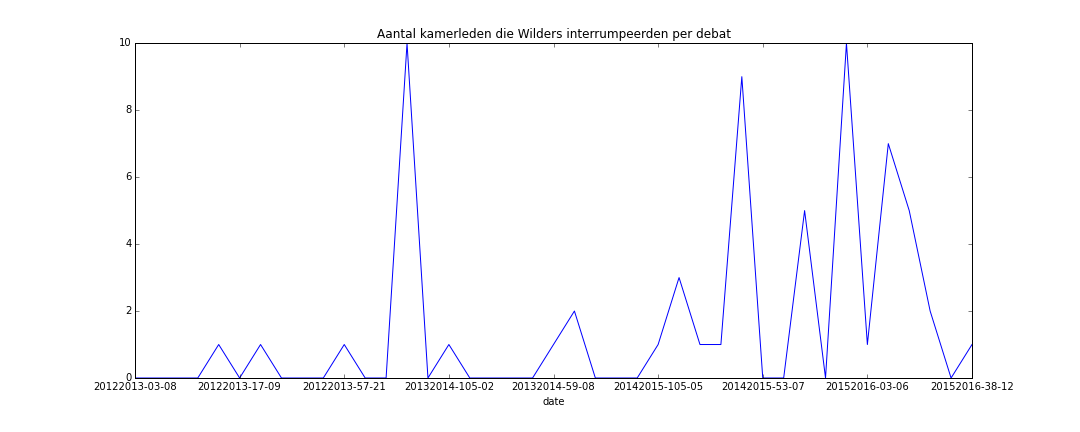
\includegraphics[width=\linewidth]{fig/WildersPlot.png}
\caption{\label{fig:wilders} Aantal interrupties van Wilders in de Tweede Kamer door de tijd (periode 2012-2016).}
\end{center}
\end{figure}


\pagebreak

\begin{table}[h]
\begin{footnotesize}
\begin{tabular}{lrl}
\toprule
{} &  indegree &                               interruptie\_volgorde \\
date            &           &                                                    \\
\midrule
20122013-03-08  &         0 &                                                    \\
20122013-07-16  &         0 &                                                    \\
20122013-100-03 &         0 &                                                    \\
20122013-100-06 &         0 &                                                    \\
20122013-17-06  &         1 &                         Pechtold-Pechtold-Pechtold \\
20122013-17-09  &         0 &                                                    \\
20122013-21-04  &         1 &                         Pechtold-Pechtold-Pechtold \\
20122013-22-08  &         0 &                                                    \\
20122013-32-06  &         0 &                                                    \\
20122013-48-23  &         0 &                                                    \\
20122013-57-21  &         1 &  Pechtold-Pechtold-Pechtold-Pechtold-Pechtold-P... \\
20122013-76-03  &         0 &                                                    \\
20122013-76-06  &         0 &                                                    \\
20132014-05-02  &        10 &  Roemer-Roemer-Van Haersma Buma-Van Haersma Bum... \\
20132014-06-04  &         0 &                                                    \\
20132014-105-02 &         1 &  Pechtold-Pechtold-Pechtold-Pechtold-Pechtold-P... \\
20132014-105-06 &         0 &                                                    \\
20132014-14-03  &         0 &                                                    \\
20132014-14-06  &         0 &                                                    \\
20132014-52-18  &         0 &                                                    \\
20132014-59-08  &         1 &                               Klaver-Klaver-Klaver \\
20142015-02-08  &         2 &  Pechtold-Pechtold-Pechtold-Pechtold-Pechtold-P... \\
20142015-03-06  &         0 &                                                    \\
20142015-09-09  &         0 &                                                    \\
20142015-100-05 &         0 &                                                    \\
20142015-105-05 &         1 &                                  Pechtold-Pechtold \\
20142015-111-04 &         3 &  Pechtold-Pechtold-Pechtold-Pechtold-Pechtold-P... \\
20142015-111-07 &         1 &                                  Pechtold-Pechtold \\
20142015-39-71  &         1 &                                  Pechtold-Pechtold \\
20142015-41-07  &         9 &  Samsom-Samsom-Pechtold-Pechtold-Pechtold-Kuzu-... \\
20142015-53-07  &         0 &                                                    \\
20142015-61-23  &         0 &                                                    \\
20142015-79-07  &         5 &  Klaver-Klaver-Klaver-Gesthuizen-Gesthuizen-Ges... \\
20142015-95-06  &         0 &                                                    \\
20152016-02-07  &        10 &  Pechtold-Pechtold-Pechtold-Pechtold-Slob-Slob-... \\
20152016-03-06  &         1 &       Pechtold-Pechtold-Pechtold-Pechtold-Pechtold \\
20152016-14-02  &         7 &  Klaver-Klaver-Roemer-Roemer-Roemer-Roemer-Sams... \\
20152016-14-05  &         5 &  Van Haersma Buma-Van Haersma Buma-Van Haersma ... \\
20152016-27-03  &         2 &  Segers-Segers-Segers-Segers-Kuzu-Kuzu-Kuzu-Kuz... \\
20152016-38-10  &         0 &                                                    \\
20152016-38-12  &         1 &                                        Klein-Klein \\
\bottomrule
\end{tabular}

\end{footnotesize}
\caption{\label{tab:Wilders} Door wie werd Wilders onderbroken en hoe vaak per debat.}
\end{table}


\pagebreak
\subsection{Methods}
Hoe je je vraag gaat beantwoorden.


Dit is de langste sectie van je scriptie. 

Als iets erg technisch wordt kan je een deel naar de Appendix verplaatsen. 

Probeer er een lopend verhaal van te maken.

Het is heel handig dit ook weer op te delen nav je deelvragen:

\subsubsection{RQ1}

\subsubsection{RQ2}